\documentclass[a4paper]{article}
% -------------------------------PACKAGES-------------------------------
\usepackage{amsmath,amsfonts,amssymb}   % for math
\usepackage{indentfirst}    % for indenting first para after section
\usepackage{xcolor}         % for coloured text
\usepackage{listings}       % for Python text
\usepackage{graphicx}       % for images
\usepackage{wrapfig}        % for wrapping images
\usepackage{hyperref}       % for hyperlinks & internal references
\usepackage[utf8]{inputenc} % for best practice
\setlength{\parskip}{1em}   % length between paras

% Change margins to components table
\usepackage{geometry}
 \geometry{
 a4paper,
 top=25mm,
 bottom=25mm,
 left=27mm,
 right=27mm,
 }
 
% Boilerplate
\title{CAB202 Microprocessors and Digital Systems\vspace{-3ex}}
\author{Johnny Madigan}
\date{\vspace{-3ex}October 2020\vspace{20ex}}

\begin{document}
\maketitle
\begin{center}

\includegraphics[width=3cm]{flower.png}
\end{center}
\newpage
\tableofcontents
\newpage

% ---------------------INTRODUCTION---------------------
\section{Introduction}\label{sec:introduction}
\par The effect of music is often overlooked, how certain combinations of sounds can influence human emotions; which is where the \emph{Undertale} Music box comes in. This music box was designed to relax people and entertain those who are familiar with \emph{Undertale}'s OST. The \emph{Undertale} theme is riddled throughout the device giving it character and further amplifying the need for its (8) functionalities.

\subsection{Functionalities}

\begin{center}
\begin{tabular}{ l | p{0.69\linewidth} }
\textbf{Functionality} & \textbf{Description}\\
 \hline
 Digital I/O (Switch) & The pushbutton provides the core interaction between the user and the device. Pressing the button starts the piezo melody and the timer, sends outputs to the serial monitor, lights up the LEDs, animates the LCD, reads the potentiometer and uses its analogue value to update the tempo. The button is controlled by a debouncing mechanism. \\\\
 Digital I/O (Debouncing) & A software debouncing mechanism is used to delay each button press by 1 millisecond to prevent mechanical noise. This may be simple, yet it is the perfect implementation for this particular device. It is necessary to allow the music to play only once without being overlapped or interrupted. Waiting 1 millisecond after each press means the button cannot be spammed.\\\\
 Digital I/O (LED) & LEDs are needed to provide a visual representation of which note is playing. This is achieved by configuring each LED’s corresponding port for output. The colourful selection of LEDs matches the theme.\\\\
 Analog Input (ADC) & Songs can easily be sped up or slowed down on computers, therefore it is vital that the music box can do the same. This is cleverly achieved by using the ADC to read a potentiometer value to update the tempo in real time.\\\\ 
 LCD & The LCD is needed to display the dancing \emph{Undertale} flower animation. This is achieved by creating custom character bitmaps, setting the cursor, and writing these custom characters on top of each other.\\\\
 Timers & \textbf{*Other than debouncing}. A core feature of the program is to capture and display timestamps of when each note is played within the overall time the device is running. Capturing these timestamps was done by enabling Timer2, a timer overflow, and turning on interrupts.\\\\
 Serial I/O (UART) & In order for the timestamps to be user-friendly, they need to be displayed. This is achieved by initiating the UART and sending timestamp Strings to the Serial Monitor. This allows users to see how they are changing the tempo in real-time. Also allows messages to be printed.\\\\
 Music synthesis tool & \textbf{*No tone library was used}. Instead, to play a note, the piezo port is configured for output and the bits are set to create a sound. The sound is then delayed for specific times to create specific tones. Therefore, each note constant holds a delayed value (integer) that has a frequency equivalent. This frequency is what I used to determines the note’s tone. Here is the documentation that provides the values to generate the desired sounds: \url{https://www.arduino.cc/en/tutorial/melody}\\\\
 \hline
\end{tabular}
\end{center}

\newpage
\subsection{Schematic}
\begin{center}
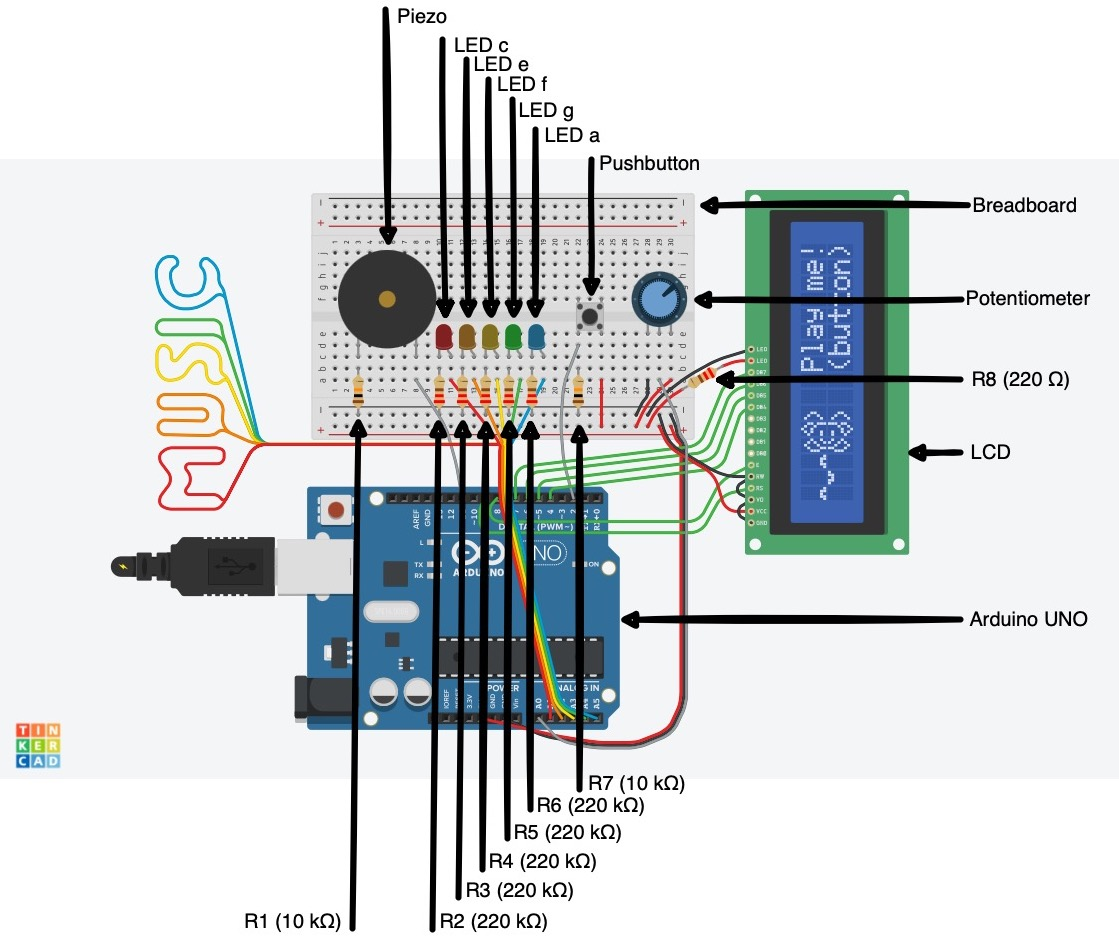
\includegraphics[width=15.5cm]{schematic.jpg}
\end{center}

\par \textbf{*Notes:} Optional "MUSIC" wire art on the left. LCD wires are all green. Positive wires are red, negative wires are black. Grey wires connect interactive components (piezo, pushbutton, and potentiometer) to the Arduino UNO. All LED wires are colour-coded to match the colour of the LEDs. The overall presentation of the diagram was designed to not only be aesthetic, but easy for anyone to re-assemble the application.

% ---------------------WIRING INSTRUCTIONS---------------------
\newpage
\section{Wiring Instructions}\label{sec:instructions}
\subsection{Set up}

\begin{wrapfigure}{r}{0.15\textwidth}
  \vspace{-25pt}
  \begin{center}
    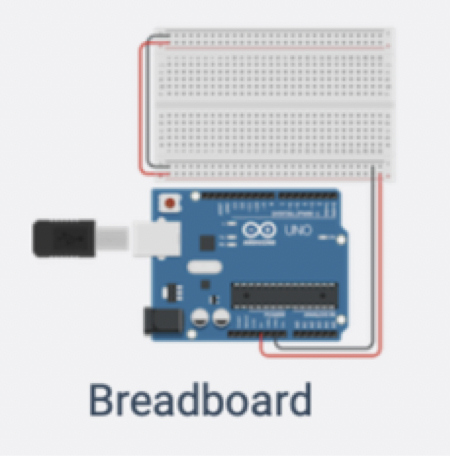
\includegraphics[width=1.1\linewidth]{breadboard.png}
  \end{center}
\vspace{-25pt}
\end{wrapfigure}

\noindent Start with an Arduino UNO R3 and a Breadboard. If using \emph{Tinkercad}, this can be found under 'Starters' then 'Arduino' then select 'Breadboard'.

\noindent \textbf{Connect the Breadboard:} Place a red wire from the power bus of the breadboard to the 5V Output of the Arduino UNO R3. Then a black wire from the ground bus of the breadboard to the ground port beside the 5V output port.

\subsection{Piezo}

\begin{wrapfigure}{r}{0.15\textwidth}
  \vspace{-50pt}
  \begin{center}
    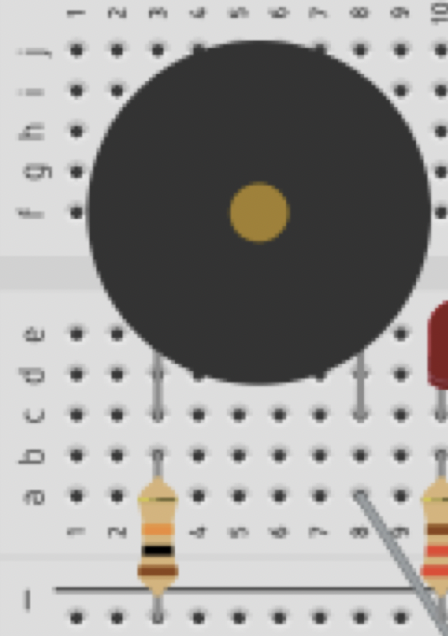
\includegraphics[width=1.1\linewidth]{piezo.png}
  \end{center}
\vspace{-25pt}
\end{wrapfigure}

\noindent \textbf{Connect the Piezo:} place the piezo on the far left of the breadboard along row c with the left contact on column 3 and the right contact on column 8; connect the right contact of the piezo to digital pin 11 with a grey wire; connect the left contact of the piezo to one end of a distinct 10 kiloOhm resistor (R1); connect the other end of the resistor to the ground bus.

\subsection{LEDs}

\begin{wrapfigure}{r}{0.15\textwidth}
  \vspace{-35pt}
  \begin{center}
    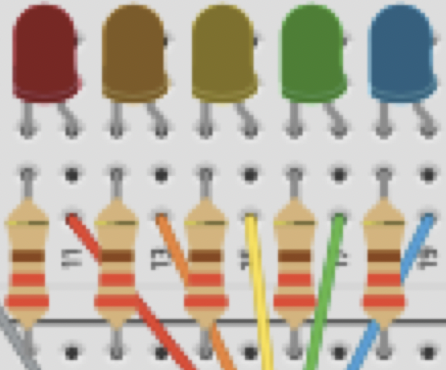
\includegraphics[width=1.1\linewidth]{leds.png}
  \end{center}
\vspace{-25pt}
\end{wrapfigure}

\noindent \textbf{Connect LED c:} place LED c (red) on the breadboard to the right of the piezo; connect digital pin 15 (analog pin 1) to the cathode of LED c; connect the anode of LED c to one end of a distinct 220 Ohm resistor (R2); connect the other end of the resistor to the ground bus.

\noindent \textbf{Connect LED e:} place LED e (orange) on the breadboard to the right of the LED c; connect digital pin 16 (analog pin 2) to the cathode of LED e; connect the anode of LED e to one end of a distinct 220 Ohm resistor (R3); connect the other end of the resistor to the ground bus.

\noindent \textbf{Connect LED f:} place LED f (yellow) on the breadboard to the right of the LED e; connect digital pin 17 (analog pin 3) to the cathode of LED f; connect the anode of LED f to one end of a distinct 220 Ohm resistor (R4); connect the other end of the resistor to the ground bus.

\noindent \textbf{Connect LED g:} place LED g (green) on the breadboard to the right of the LED f; connect digital pin 18 (analog pin 4) to the cathode of LED g; connect the anode of LED g to one end of a distinct 220 Ohm resistor (R5); connect the other end of the resistor to the ground bus.

\noindent \textbf{Connect LED a:} place LED a (blue) on the breadboard to the right of the LED g; connect digital pin 19 (analog pin 5) to the cathode of LED a; connect the anode of LED a to one end of a distinct 220 Ohm resistor (R6); connect the other end of the resistor to the ground bus.

\subsection{Pushbutton}

\begin{wrapfigure}{r}{0.15\textwidth}
  \vspace{-50pt}
  \begin{center}
    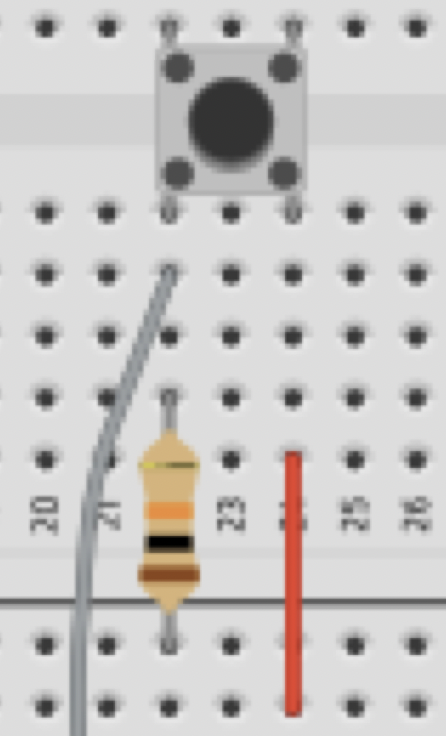
\includegraphics[width=1.1\linewidth]{pushbutton.png}
  \end{center}
\vspace{-25pt}
\end{wrapfigure}

\noindent \textbf{Connect the Pushbutton:} place the pushbutton on the breadboard to the right of LED a; connect terminal 1a of the pushbutton to digital pin 2; below that wire, connect terminal 1a of the pushbutton to one end of a distinct 10 kiloOhm resistor (R7); connect the other end of the resistor to the ground bus; connect terminal 2a of the pushbutton the power bus.

\newpage
\subsection{Potentiometer}

\begin{wrapfigure}{r}{0.15\textwidth}
  \vspace{-35pt}
  \begin{center}
    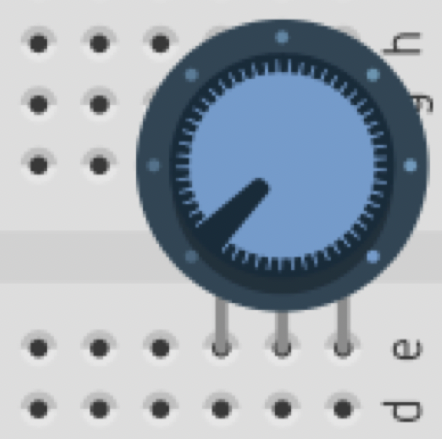
\includegraphics[width=1.1\linewidth]{potentiometer.png}
  \end{center}
\vspace{-25pt}
\end{wrapfigure}

\noindent \textbf{Connect the Potentiometer:} place the potentiometer on the far right of the breadboard to the right of the pushbutton; connect terminal 1 of the potentiometer to the ground bus; connect the wiper of the potentiometer to digital pin 14 (analog pin 0); connect terminal 2 of the potentiometer to the power bus.

\subsection{LCD}

\begin{wrapfigure}{r}{0.15\textwidth}
  \vspace{-25pt}
  \begin{center}
    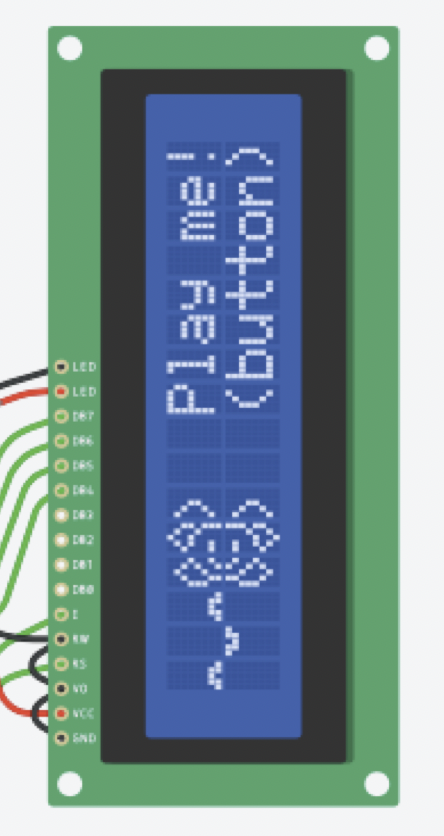
\includegraphics[width=1.1\linewidth]{lcd.png}
  \end{center}
\vspace{-25pt}
\end{wrapfigure}

\noindent \textbf{Connect the LCD’s power and ground pins:} First place an LCD vertically beside the breadboard; on the LCD connect GND (ground pin) to V0 (contrast pin); connect V0 (contrast pin) to RW (read/write pin); connect RW (read/write pin) to the ground bus on the breadboard; connect the LED Cathode pin on the LCD to the ground bus on the breadboard; connect the LED Anode pin on the LCD to one end of a distinct 220 Ohm resistor (R8); connect the other end of the resistor to the power bus on the breadboard; connect VCC (power pin) to the power bus on the breadboard.

\noindent \textbf{Connect the LCD’s other pins:} connect RS (register select pin) to digital pin 9; connect E (enable pin) to digital pin 8; connect DB7 pin to digital pin 7; connect DB6 pin to digital pin 6; connect DB5 pin to digital pin 5; connect DB4 pin to digital pin 4.

% ---------------------LINKS---------------------
\section{Links}\label{sec:links}

\subsection{Arduino Melody Documentation}

Link to the Arduino melody documentation: \url{https://www.arduino.cc/en/tutorial/melody}

\subsection{Tinkercad file}

Link to my public \emph{Tinkercad} file: \url{https://www.tinkercad.com/things/6StnqF56pt9}

\subsection{Demonstration video}

Link to my demonstration video (Oct, 2020): \url{https://www.youtube.com/watch?v=2LdCBoPOooE}

\end{document}
